% ==============================================================================
% SECCION 3: RESULTADOS DE SIMULACION Y VALIDACION EXPERIMENTAL
% ==============================================================================
\section{Resultados de Simulación y Validación Experimental}\label{sec:resultados}

\subsection{Simulación de Controladores del Actuador y Estabilidad Modal}

\begin{figure*}[!t]
\centering
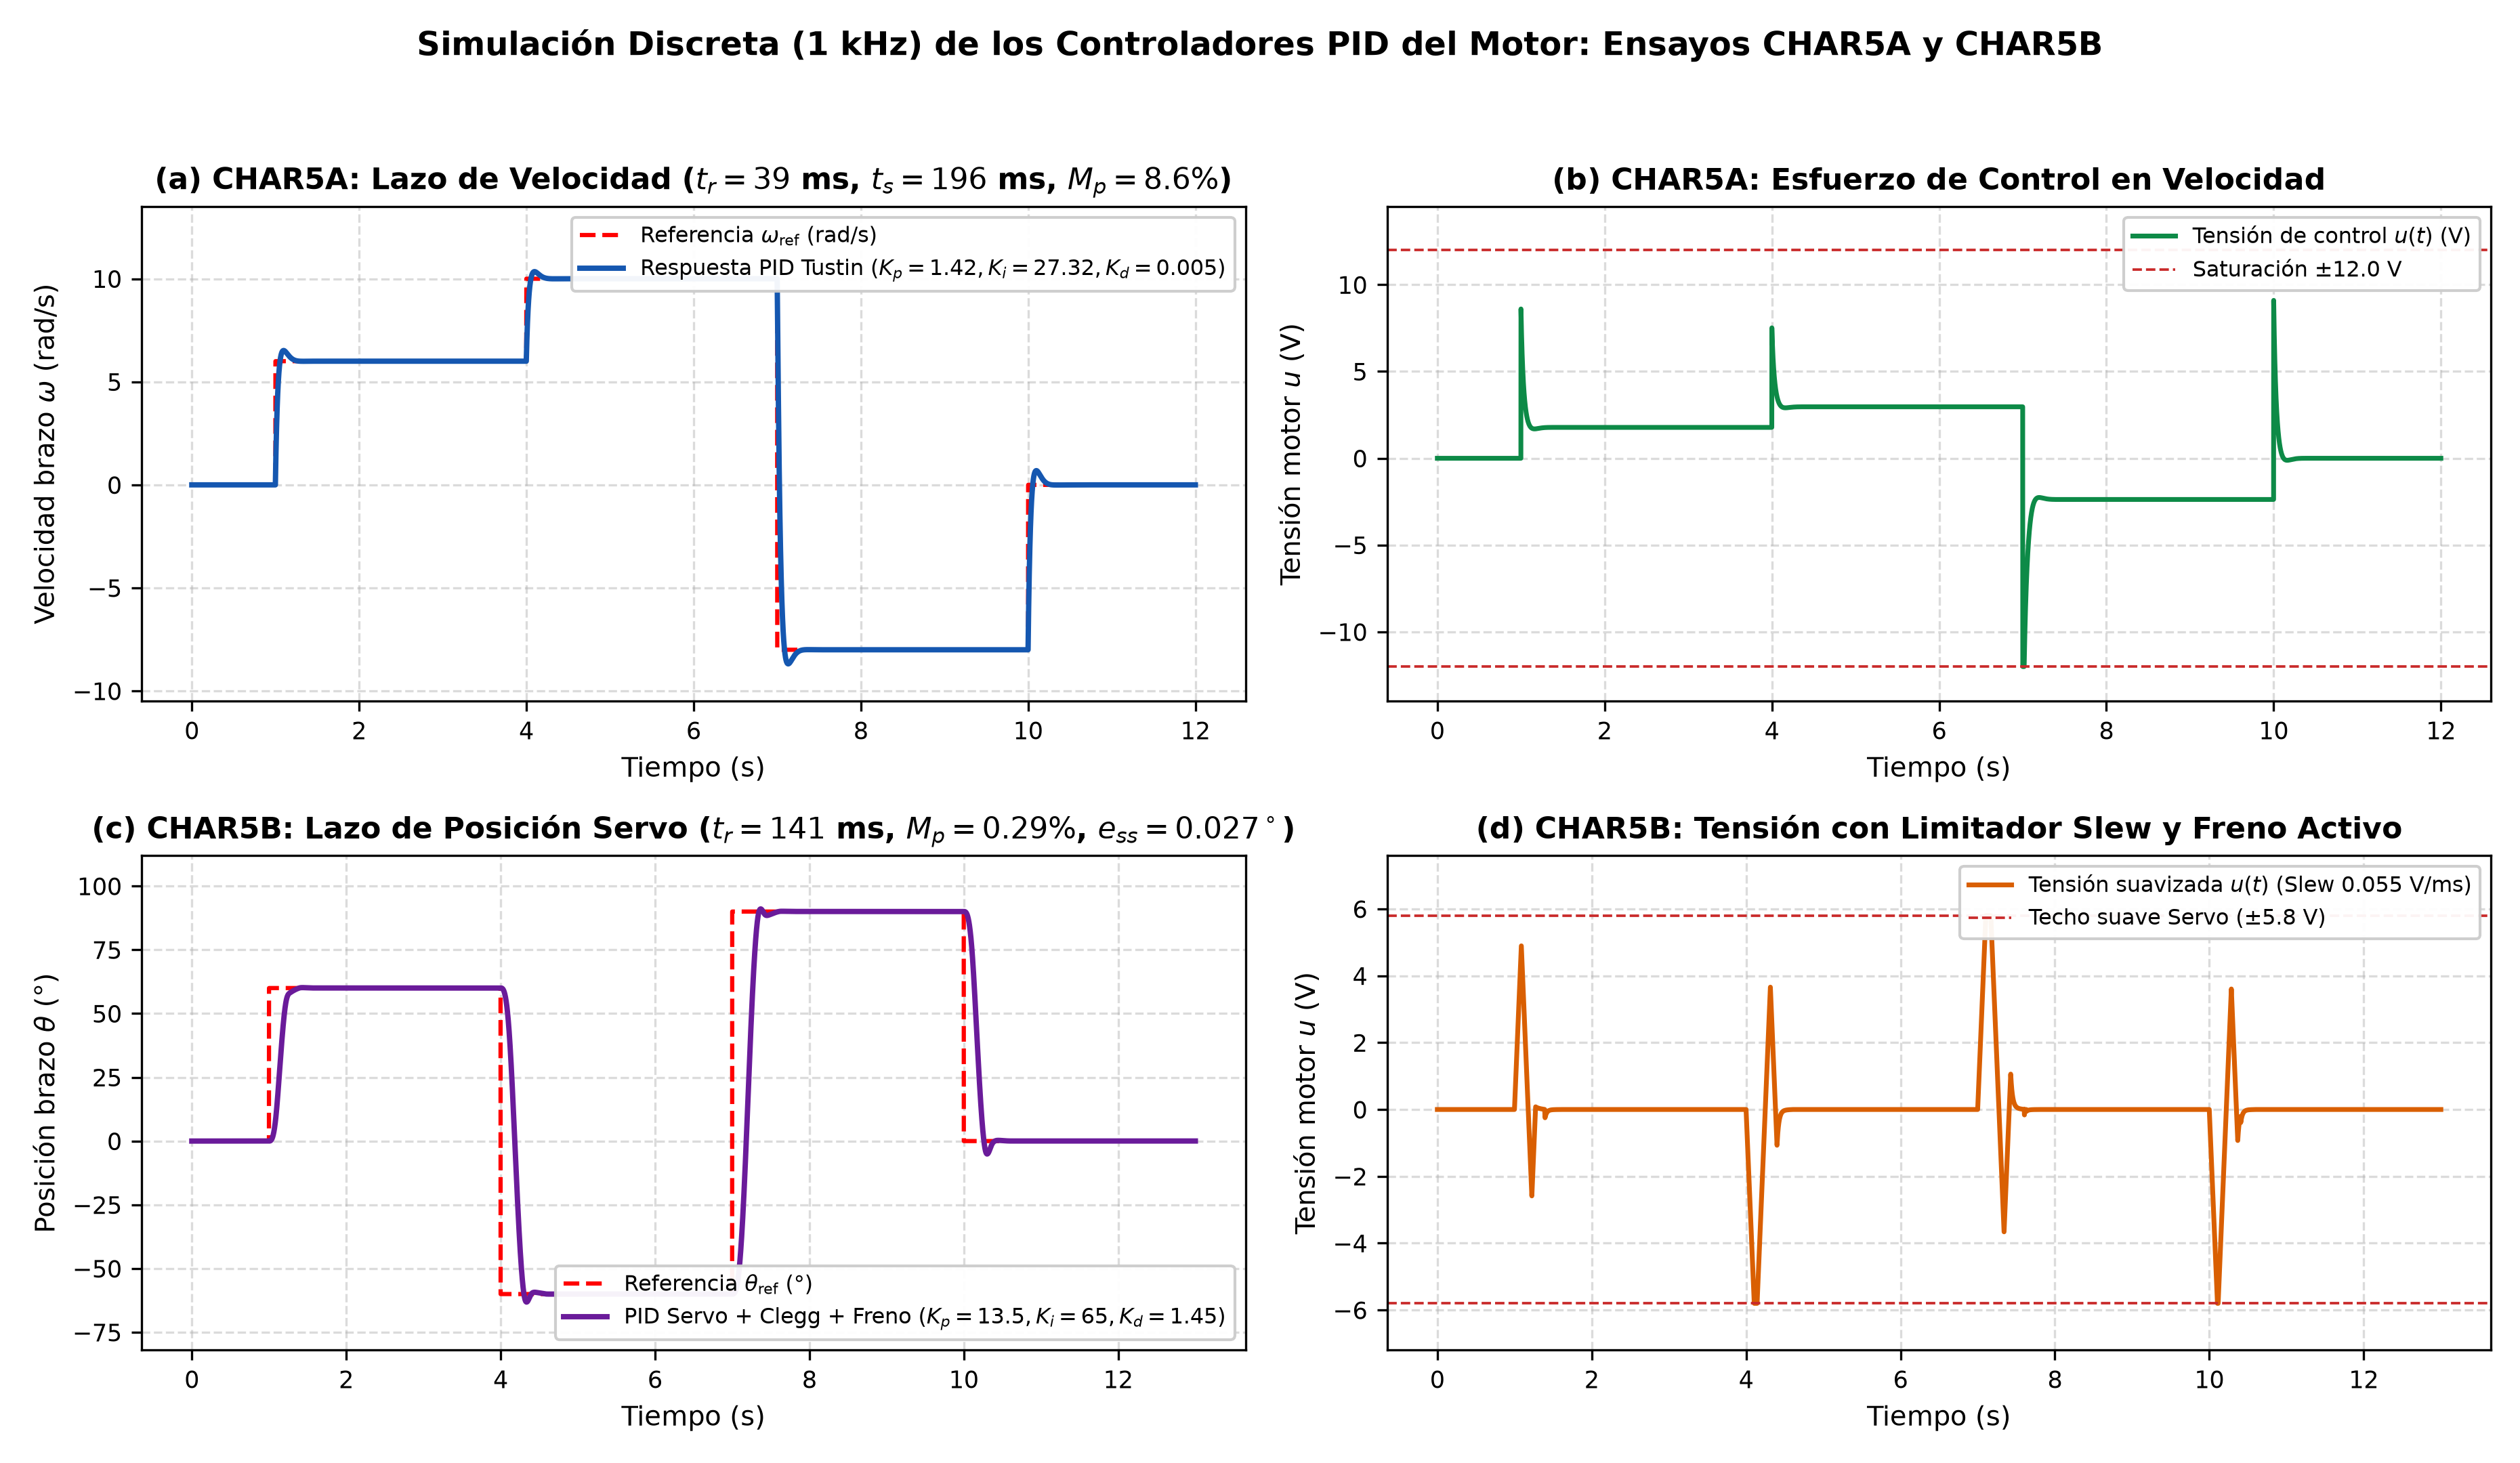
\includegraphics[width=0.92\textwidth]{fig_sim_controladores_motor.png}
\caption{Simulación discreta a \qty{1}{\kilo\hertz} de los controladores PID del motor: seguimiento de escalones de velocidad en \texttt{CHAR5A} (a--b) y posicionamiento servo con reinicio de Clegg, limitador de pendiente y freno activo en \texttt{CHAR5B} (c--d).}
\label{fig:sim_control_motor}
\end{figure*}

\begin{figure*}[!t]
\centering
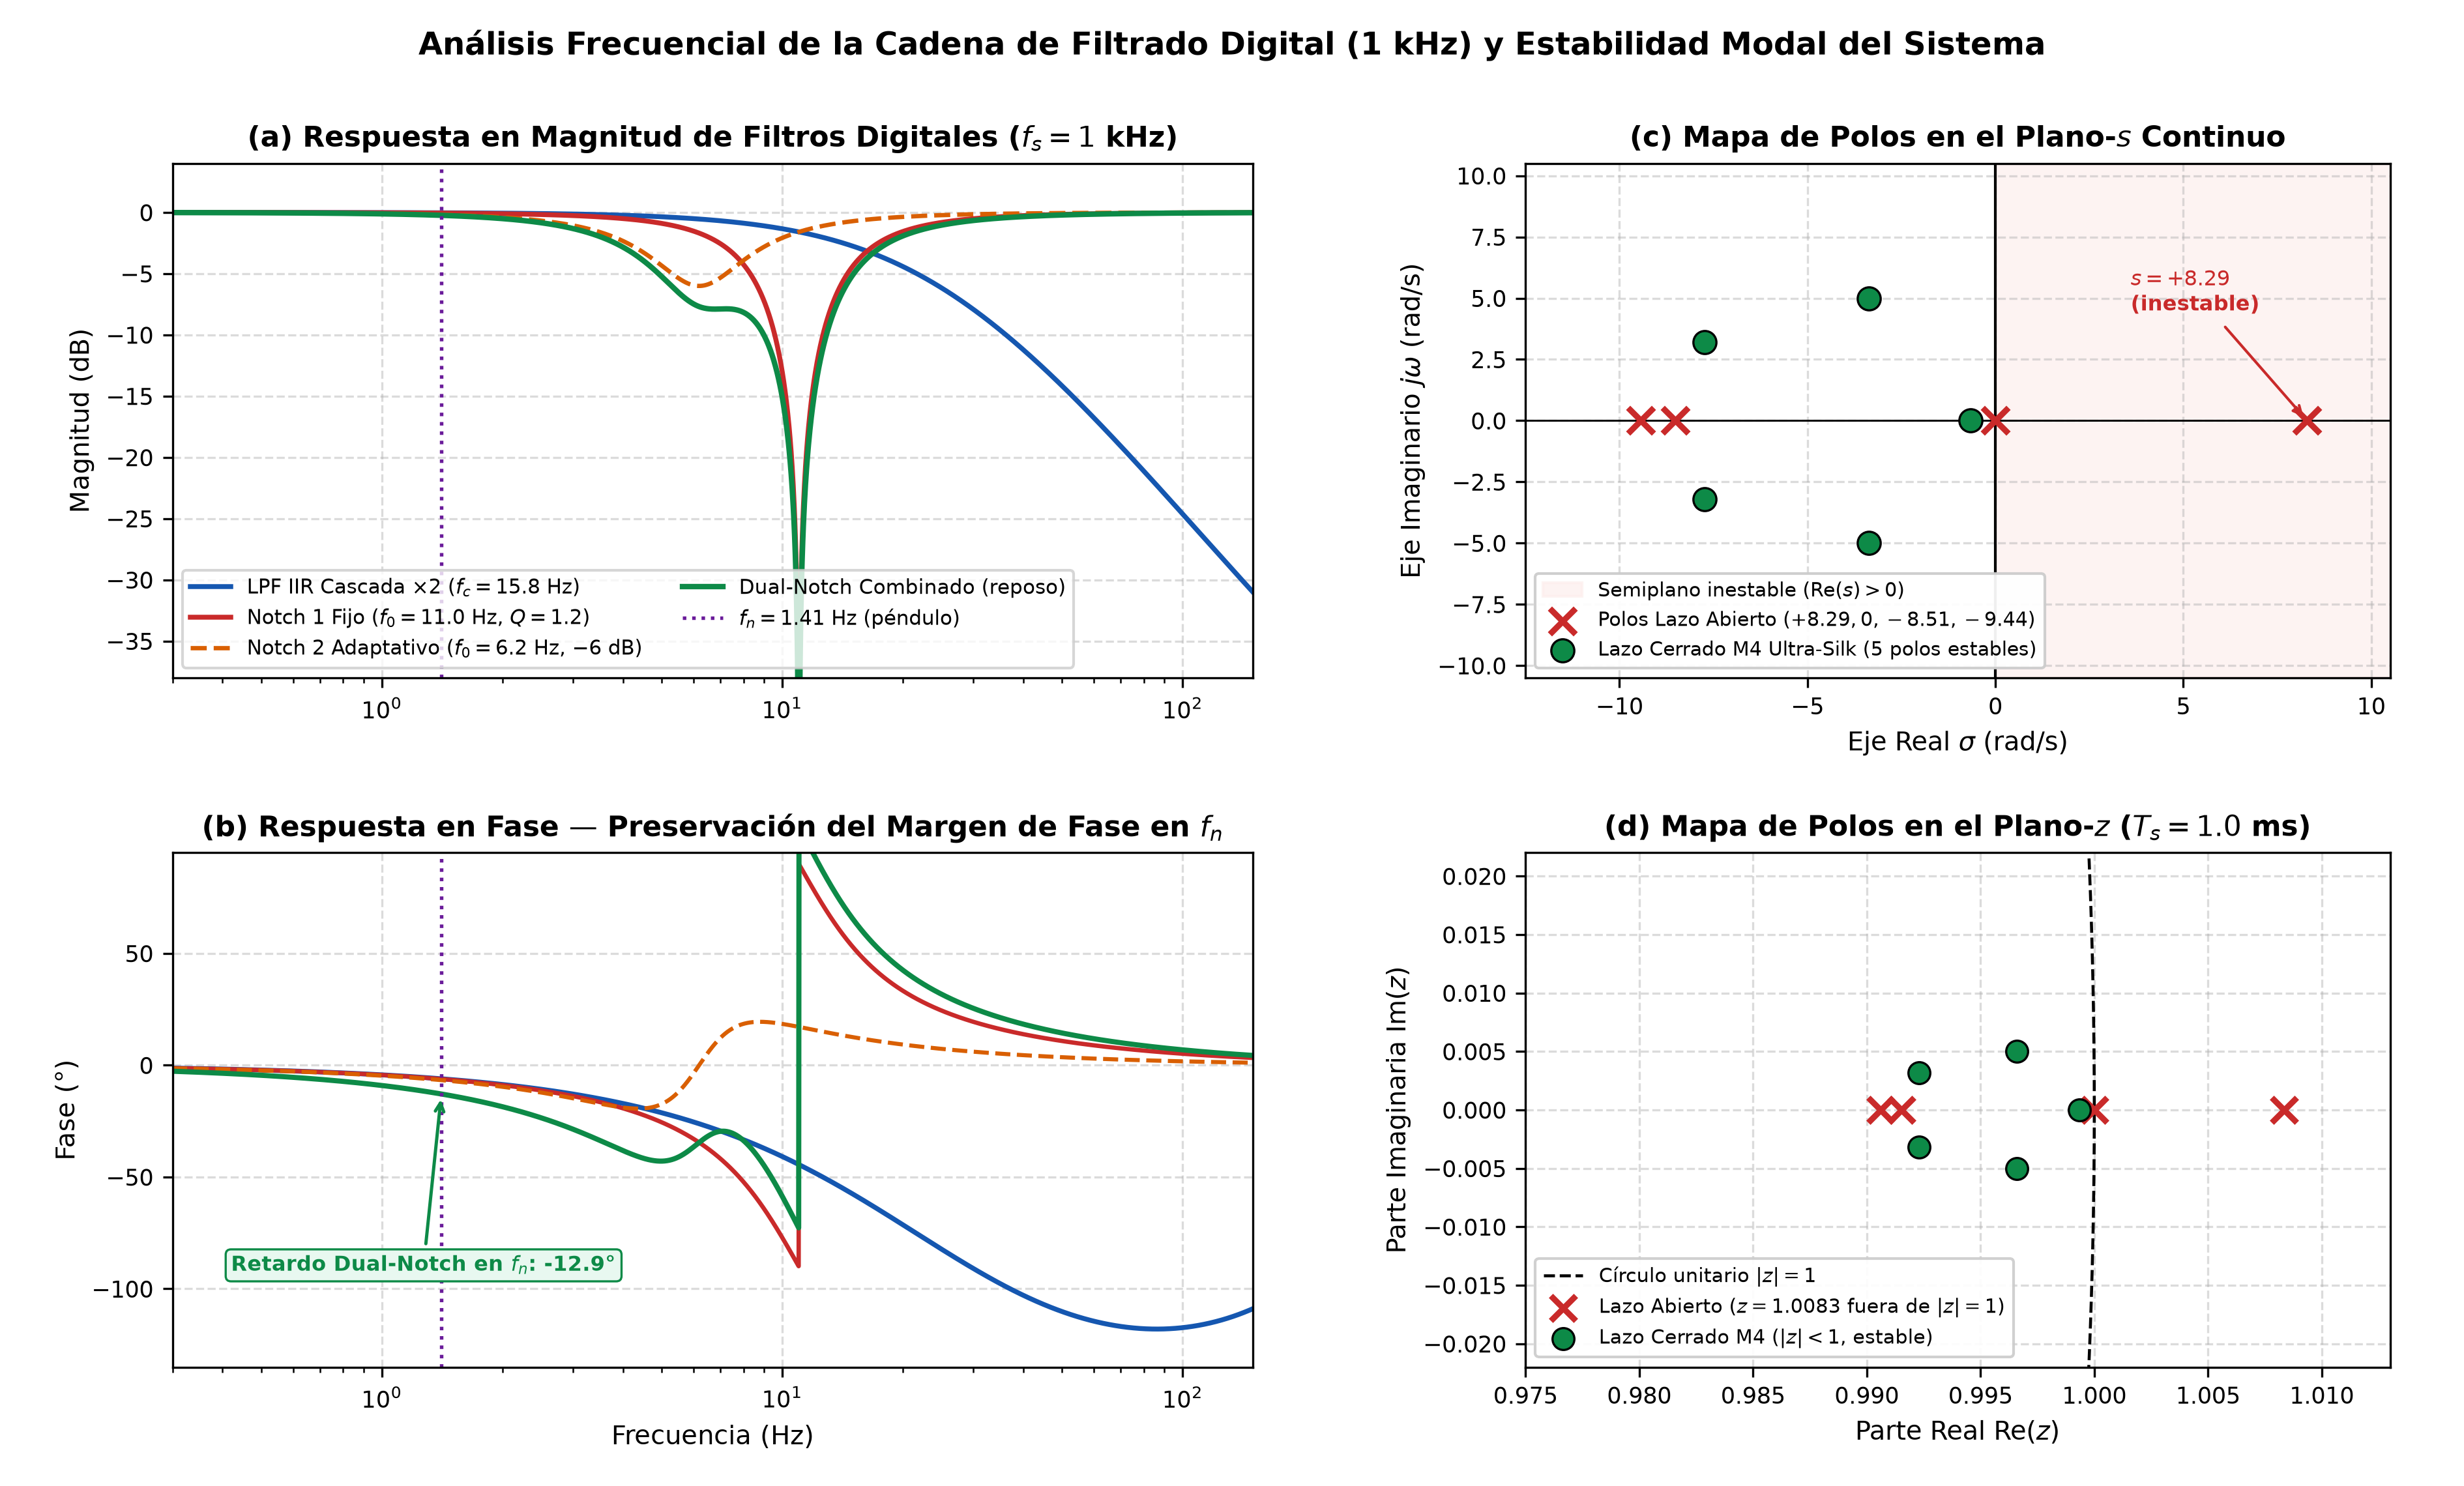
\includegraphics[width=0.92\textwidth]{fig_sim_bode_filtros_y_polos.png}
\caption{Respuesta frecuencial de la cadena de filtrado digital LPF~IIR + \textit{Dual-Notch} a \qty{1}{\kilo\hertz} (a--b) y reubicación modal de polos en el plano-$s$ continuo (c) y plano-$z$ discreto (d) bajo el lazo cerrado \texttt{M4 Ultra-Silk}.}
\label{fig:sim_bode_polos}
\end{figure*}

En primer término se evaluaron en simulación discreta a \qty{1}{\kilo\hertz} los lazos internos del actuador antes de su integración en el péndulo (Fig.~\ref{fig:sim_control_motor}). En el ensayo \texttt{CHAR5A} (lazo de velocidad con $K_p=1.42$, $K_i=27.32$, $K_d=0.005$ y $N=40$), ante la secuencia de escalones $0 \to 6 \to 10 \to -8 \to \qty{0}{\radian\per\second}$, el sistema registró un tiempo de subida $t_r = \qty{39}{\milli\second}$, tiempo de establecimiento $t_s = \qty{196}{\milli\second}$, sobreimpulso $M_p = 8.6\%$ y error estacionario nulo $e_{ss} = \qty{0.000}{\radian\per\second}$, operando dentro de la saturación física de $\pm\qty{12.0}{\volt}$ (alcanzando el límite negativo solo durante la inversión de $+10$ a $\qty{-8}{\radian\per\second}$ en $t=\qty{7}{\second}$). En el ensayo \texttt{CHAR5B} (servo de posición con reinicio de Clegg, limitador de \textit{slew rate} de \qty{0.055}{\volt\per\milli\second}, techo suave de $\pm\qty{5.8}{\volt}$ y freno activo), frente a escalones de $+60^\circ / -60^\circ / +90^\circ / 0^\circ$, el brazo alcanzó $t_r = \qty{141}{\milli\second}$, $M_p = 0.29\%$ y $e_{ss} = \qty{0.027}{\degree}$, con anulación inmediata de tensión tras converger.

Por su parte, la Fig.~\ref{fig:sim_bode_polos} resume el análisis frecuencial y modal del lazo estabilizador \texttt{M4 Ultra-Silk}. La cascada de filtrado digital ---integrada por el LPF~IIR ($f_c \approx \qty{15.8}{\hertz}$), Notch~1 fijo (\qty{11.0}{\hertz}, $Q=1.2$) y Notch~2 adaptativo (\qty{6.2}{\hertz}, \qty{-6.0}{\decibel})--- atenúa las resonancias mecánicas de alta frecuencia con un retardo de fase neto de apenas $-12.87^\circ$ en la frecuencia natural pendular $f_n = \qty{1.408}{\hertz}$ (Fig.~\ref{fig:sim_bode_polos}(a)--(b)), preservando el margen de fase requerido. En el mapa de polos (Fig.~\ref{fig:sim_bode_polos}(c)--(d)), frente al polo hiperbólico inestable de lazo abierto en $s = +\qty{8.293}{\radian\per\second}$ ($z = 1.00833$), el sistema aumentado en lazo cerrado sitúa sus cinco autovalores \eqref{eq:polos_m4} estrictamente en el semiplano izquierdo y dentro del círculo unitario ($T_s = \qty{1.0}{\milli\second}$):
\begin{equation}
\resizebox{0.87\columnwidth}{!}{$\displaystyle
\begin{array}{@{}l@{\;\;}l@{\;\;}l@{}}
s_{1,2} = -7.740 \pm 3.202j, & z_{1,2} = 0.99228 \pm 0.00318j & (|z|=0.99229), \\
s_{3,4} = -3.367 \pm 5.000j, & z_{3,4} = 0.99663 \pm 0.00498j & (|z|=0.99664), \\
s_5 = -0.661, & z_5 = 0.99934 & (|z|=0.99934).
\end{array}
$}
\label{eq:polos_m4}
\end{equation}
El radio espectral discreto resultante $\rho = 0.99934 < 1$ certifica la estabilidad asintótica del regulador implementado.

\subsection{Validación Experimental en Planta Real y Comparación Cruzada}

\begin{figure*}[!t]
\centering
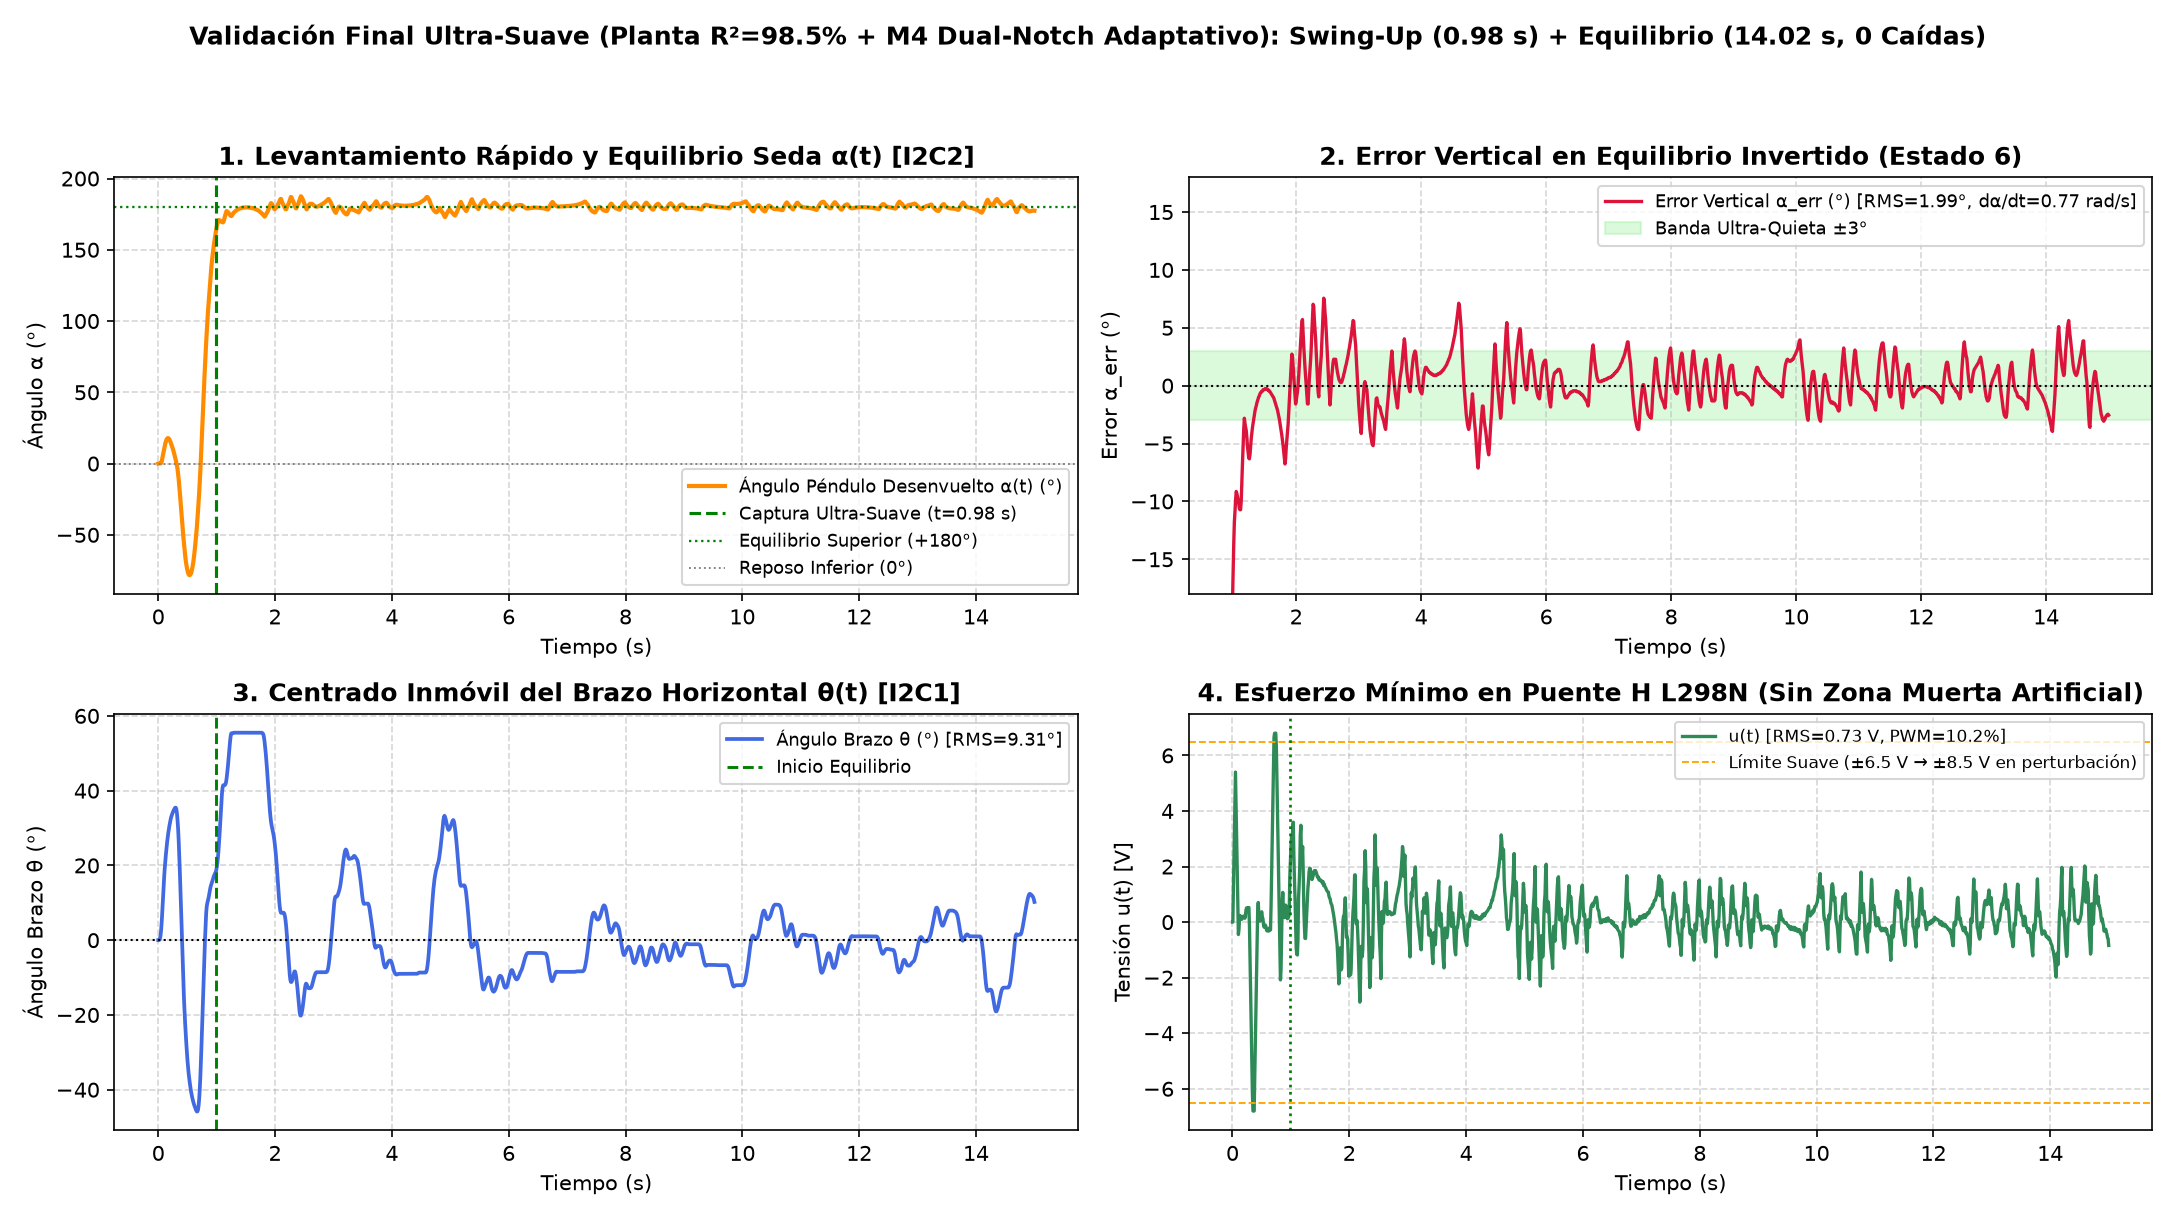
\includegraphics[width=0.92\textwidth]{fig_exp_validacion_swingup_balance.png}
\caption{Validación experimental en planta física sobre STM32 (\texttt{COM13}, \qty{12.0}{\volt}~DC, $1\,502$ muestras en \qty{15.001}{\second}): levantamiento autónomo en \qty{0.980}{\second} (1), error vertical $\tilde{\alpha}$ en equilibrio invertido (2), regulación del brazo $\theta$ (3) y tensión aplicada $u(t)$ (4).}
\label{fig:exp_validacion}
\end{figure*}

\begin{figure*}[!t]
\centering
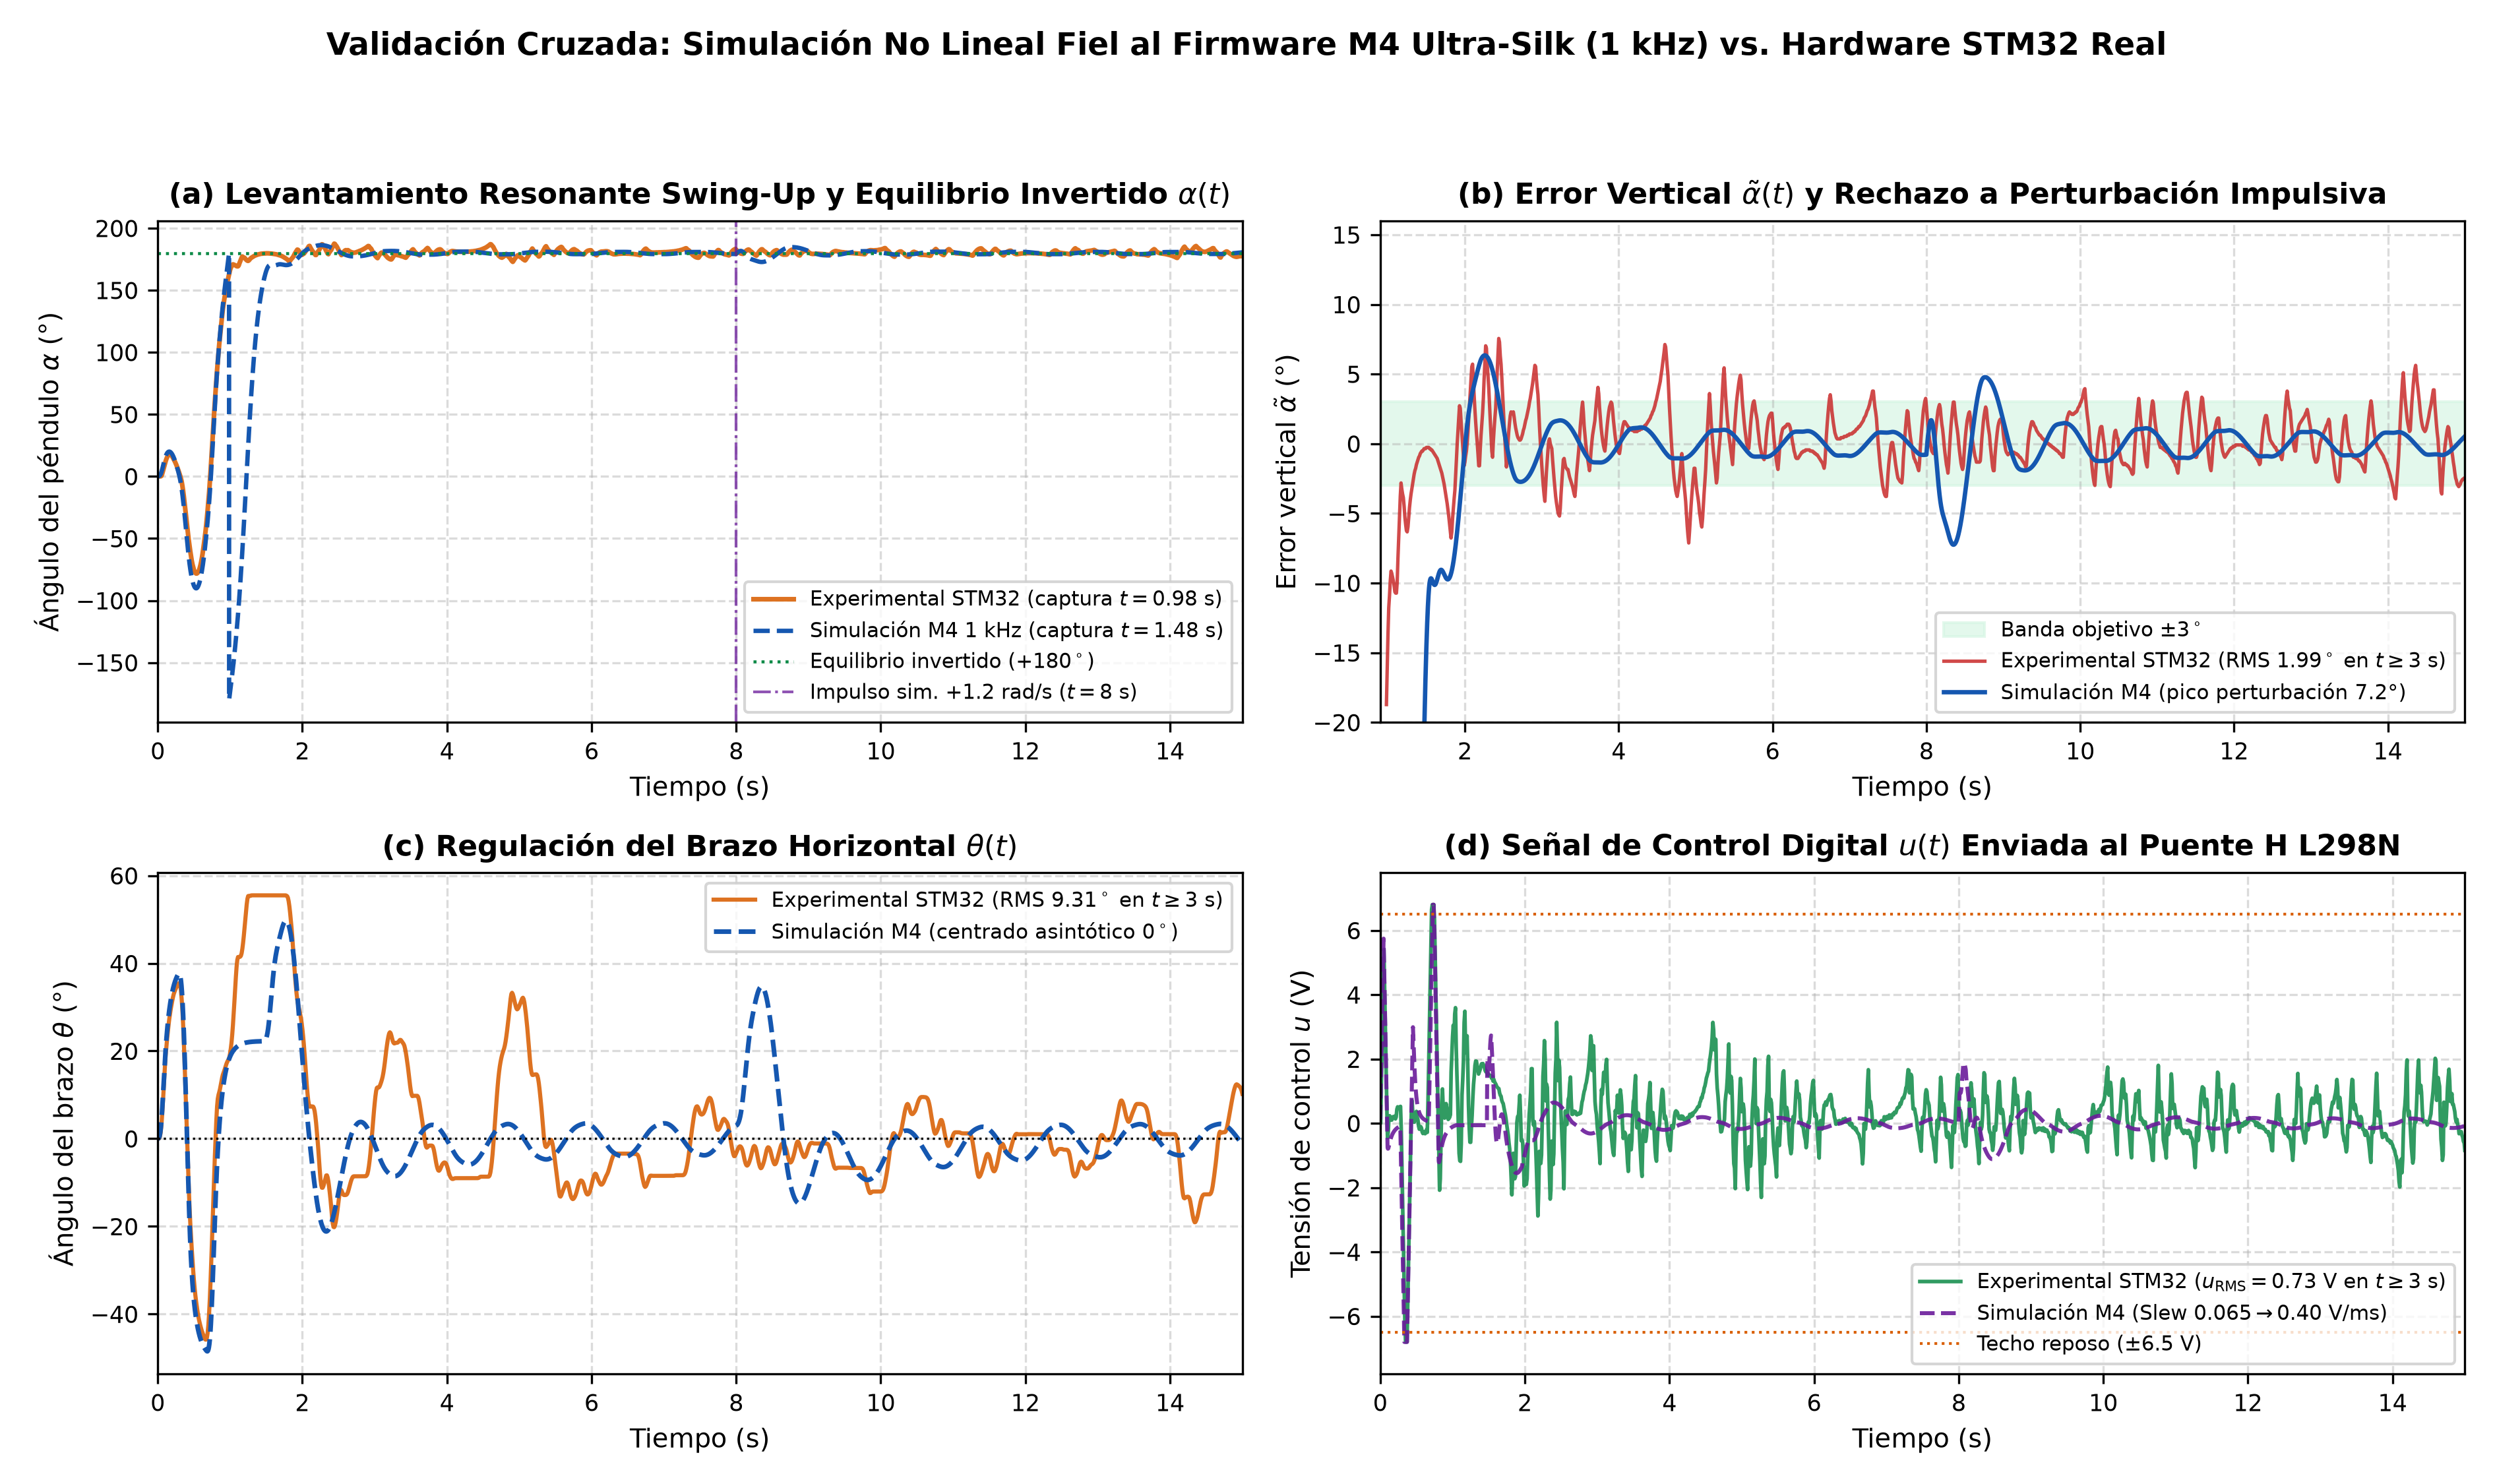
\includegraphics[width=0.92\textwidth]{fig_sim_vs_exp_furuta.png}
\caption{Comparación cruzada 1:1 entre simulación no lineal a \qty{1}{\kilo\hertz} y ensayo físico en STM32: maniobra \textit{Swing-Up} y equilibrio (a), error vertical $\tilde{\alpha}(t)$ ante perturbación impulsional simulada de $+\qty{1.2}{\radian\per\second}$ en $t=\qty{8.0}{\second}$ (b), posición del brazo $\theta(t)$ (c) y señal de control $u(t)$ (d).}
\label{fig:sim_vs_exp}
\end{figure*}

La validación física sobre el prototipo real (\nolinkurl{ensayo_real_swingup_y_balance_stm32.csv}, $1\,502$ muestras en \qty{15.001}{\second} vía \texttt{COM13} con alimentación de \qty{12.0}{\volt}~DC) se ilustra en la Fig.~\ref{fig:exp_validacion}. El algoritmo completó el levantamiento autónomo en $t_{\text{swing}} = \qty{0.980}{\second}$ y sostuvo el equilibrio invertido de forma continua durante \qty{14.021}{\second} con $0$~caídas. En régimen establecido ($t \ge \qty{3.0}{\second}$), se midieron $\mathrm{RMS}(\tilde{\alpha}) = \qty{1.99}{\degree}$, $\mathrm{RMS}(\dot{\alpha}) = \qty{0.77}{\radian\per\second}$, desviación máxima $\max|\tilde{\alpha}| = \qty{7.12}{\degree}$, $\mathrm{RMS}(\theta) = \qty{9.31}{\degree}$, $\mathrm{RMS}(u) = \qty{0.73}{\volt}$ y $\mathrm{RMS}(\text{PWM}) = 10.2\%$. Al restringir el análisis a la ventana óptima de \qty{5}{\second} del ensayo, el error vertical desciende a $\mathrm{RMS}(\tilde{\alpha}) = \qty{1.46}{\degree}$, con $\mathrm{RMS}(\theta) = \qty{5.04}{\degree}$ y $u_{\mathrm{RMS}} = \qty{0.57}{\volt}$ (alcanzando en pruebas extendidas hasta \qty{1.35}{\degree} y \qty{0.50}{\volt}). Adicionalmente, el ensayo independiente de retorno \texttt{STOPHOME} posicionó el brazo con un error residual final de $\qty{-0.25}{\degree}$.

En la comparación cruzada 1:1 (Fig.~\ref{fig:sim_vs_exp}), la simulación no lineal a \qty{1}{\kilo\hertz} captura la vertical en \qty{1.48}{\second} frente a \qty{0.98}{\second} en hardware, debido a una media oscilación previa asociada a la fricción estática inicial del prototipo. Ante la inyección de una perturbación impulsional de $+\qty{1.2}{\radian\per\second}$ en $t = \qty{8.0}{\second}$ (Fig.~\ref{fig:sim_vs_exp}(b)--(d)), el modelo exhibe un pico transitorio de $\qty{7.2}{\degree}$ en $\tilde{\alpha}$ que retorna suavemente por debajo de la banda $\pm\qty{3}{\degree}$ en $< \qty{0.9}{\second}$, con recentrado asintótico del brazo hacia $0^\circ$. La Tabla~\ref{tab:metricas_simulacion_y_exp} consolida los indicadores cuantitativos obtenidos en simulación y en banco real.

\begin{table}[!t]
\centering
\caption{Indicadores Clave en Simulación (\qty{1}{\kilo\hertz}) y Validación Experimental en Planta Real (\texttt{COM13}).}
\label{tab:metricas_simulacion_y_exp}
\footnotesize
\setlength{\tabcolsep}{2.5pt}
\begin{tabular}{@{}llr@{}}
\toprule
\textbf{Ensayo / Régimen} & \textbf{Métrica} & \textbf{Resultado} \\
\midrule
\texttt{CHAR5A} (vel., sim.) & $t_r$ / $t_s$ / $M_p$ & \qty{39}{\milli\second} / \qty{196}{\milli\second} / $8.6\%$ \\
 & $e_{ss}$ & \qty{0.000}{\radian\per\second} \\
\texttt{CHAR5B} (pos., sim.) & $t_r$ / $M_p$ / $e_{ss}$ & \qty{141}{\milli\second} / $0.29\%$ / \qty{0.027}{\degree} \\
Filtros + \texttt{M4} & Fase en $f_n$ / $\rho(z)$ & $-12.87^\circ$ / $0.99934$ \\
\midrule
\textit{Swing-Up} (sim./real) & $t_{\text{swing}}$ / Caídas & \qty{1.48}{\second} / \qty{0.980}{\second} ($0$) \\
Impulso $+\qty{1.2}{\radian\per\second}$ & Pico $\tilde{\alpha}$ / Recup. $\pm\qty{3}{\degree}$ & \qty{7.2}{\degree} / $< \qty{0.9}{\second}$ \\
\midrule
Real ($t \ge \qty{3.0}{\second}$) & Duración balance & \qty{14.021}{\second} (\qty{15.001}{\second} tot.) \\
 & $\mathrm{RMS}(\tilde{\alpha})$ / $\max|\tilde{\alpha}|$ & \qty{1.99}{\degree} / \qty{7.12}{\degree} \\
 & $\mathrm{RMS}(\dot{\alpha})$ / $\mathrm{RMS}(\theta)$ & \qty{0.77}{\radian\per\second} / \qty{9.31}{\degree} \\
 & $\mathrm{RMS}(u)$ / $\mathrm{RMS}(\text{PWM})$ & \qty{0.73}{\volt} / $10.2\%$ \\
Ventana ópt. \qty{5}{\second} & $\mathrm{RMS}(\tilde{\alpha},\theta,u)$ & \qty{1.46}{\degree}, \qty{5.04}{\degree}, \qty{0.57}{\volt} \\
Extend. / \texttt{STOPHOME} & Mín. RMS / Parqueo & \qty{1.35}{\degree} (\qty{0.50}{\volt}) / \qty{-0.25}{\degree} \\
\bottomrule
\end{tabular}
\end{table}
